\documentclass[tikz,border=4pt]{standalone}
% Estilo común de los diagramas de bloques (se usa con \input en cada standalone)
\usepackage[defaultsans,scale=0.92]{lato}
\usepackage{libertinust1math}
\usepackage{xcolor,amsmath}
\usepackage{tikz}
\usetikzlibrary{positioning,arrows.meta,calc,shapes.geometric}
\usepackage{../../notacion}
\definecolor{ctrlazul}{HTML}{1E5AA8}\definecolor{ctrlnoche}{HTML}{14213D}
\definecolor{ctrlcoral}{HTML}{D1495B}\definecolor{ctrlverde}{HTML}{2A9D8F}
\definecolor{ctrlambar}{HTML}{E09F3E}\definecolor{ctrlgris}{HTML}{5C677D}
\definecolor{ctrlvioleta}{HTML}{6C4AB6}\definecolor{ctrlteal}{HTML}{0F7173}
\tikzset{
  >={Stealth[length=2.4mm]}, every node/.style={font=\small},
  bloque/.style={draw=ctrlnoche,fill=ctrlazul!7,thick,rounded corners=1.5pt,minimum height=9mm,minimum width=13mm,inner sep=4pt},
  suma/.style={draw=ctrlnoche,thick,circle,inner sep=0pt,minimum size=6mm},
  senal/.style={->,thick,draw=ctrlnoche},
  rot/.style={font=\footnotesize,text=ctrlgris},
}

\begin{document}
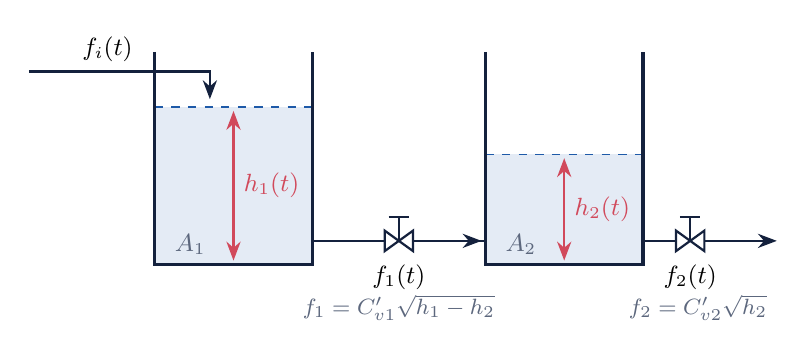
\begin{tikzpicture}[font=\small,
  valvula/.pic={\draw[thick,ctrlnoche,fill=white] (-0.18,-0.13)--(0.18,0.13)--(0.18,-0.13)--(-0.18,0.13)--cycle; \draw[thick,ctrlnoche] (0,0)--(0,0.3) (-0.13,0.3)--(0.13,0.3);}]
  % tanque 1
  \fill[ctrlazul!12] (0,0) rectangle (2,2.0); \draw[ctrlazul,dashed] (0,2.0)--(2,2.0);
  \draw[very thick,ctrlnoche] (0,2.7)--(0,0)--(2,0)--(2,2.7);
  \draw[<->,ctrlcoral,thick] (1,0.05)--(1,1.95) node[midway,right]{$h_1(t)$};
  \node[ctrlgris] at (0.45,0.25) {$A_1$};
  % tanque 2
  \begin{scope}[xshift=4.2cm]
  \fill[ctrlazul!12] (0,0) rectangle (2,1.4); \draw[ctrlazul,dashed] (0,1.4)--(2,1.4);
  \draw[very thick,ctrlnoche] (0,2.7)--(0,0)--(2,0)--(2,2.7);
  \draw[<->,ctrlcoral,thick] (1,0.05)--(1,1.35) node[midway,right]{$h_2(t)$};
  \node[ctrlgris] at (0.45,0.25) {$A_2$};
  \end{scope}
  % entrada
  \draw[senal] (-1.6,2.45)--(0.7,2.45)--(0.7,2.1); \node[above] at (-0.6,2.45) {$f_i(t)$};
  % válvula 1
  \draw[thick,ctrlnoche] (2,0.3)--(4.2,0.3); \draw[senal] (3.5,0.3)--(4.15,0.3);
  \pic at (3.1,0.3) {valvula}; \node[below] at (3.1,0.12) {$f_1(t)$};
  % válvula 2
  \draw[thick,ctrlnoche] (6.2,0.3)--(7.6,0.3); \draw[senal] (7.0,0.3)--(7.9,0.3);
  \pic at (6.8,0.3) {valvula}; \node[below] at (6.8,0.12) {$f_2(t)$};
  \node[rot] at (3.1,-0.55) {$f_1=C'_{v1}\sqrt{h_1-h_2}$};
  \node[rot] at (6.9,-0.55) {$f_2=C'_{v2}\sqrt{h_2}$};
\end{tikzpicture}
\end{document}
